\chapter{Fundamentos generales}
En este capítulo se desarrollan las bases matemáticas de los distintos algoritmos a implementar.
\section{Introducción}
Los algoritmos de cifrado asimétrico analizados en este Trabajo Fin de Grado corresponden a mecanismos de intercambio de claves (\gls{kem}), es decir, procedimientos diseñados para establecer un secreto compartido entre dos partes. Este secreto se utiliza posteriormente como clave en algoritmos de cifrado simétrico, con el fin de garantizar una comunicación segura, ya que este tipo de cifrado requiere que ambas partes dispongan previamente de una misma clave secreta.
\newline

Siguiendo las recomendaciones del \gls{nist} \cite{NIST_SP_800_227_ipd_2025}, uno de los enfoques consiste en establecer dichas claves a través de un canal público de comunicaciones. Para ello, de forma general y en el contexto de los algoritmos considerados en este trabajo, se emplea un esquema como el ilustrado en la figura \ref{fig:mainprotocol} donde Alice y Bob intercambian las claves mediante tres pasos:
\begin{enumerate}
	\item \textbf{Generación de llaves}: se generan una llave privada, que Alice debe mantener en secreto para no comprometer la seguridad del protocolo, y una llave pública, derivada de la privada, que Alice enviará a Bob.
	\item \textbf{Encapsulado}: Bob, usando valores la llave pública de Alice, genera un ciphertexto que enviará a Alice y el secreto compartido.
	\item \textbf{Decapsulado}: Alice, a partir del ciphertexto recibido y su llave privada, deriva el mismo secreto compartido que Bob.
\end{enumerate}


Por último, es importante señalar que existe un paso adicional denominado confirmación de claves, con el objetivo de verificar que ambas partes han obtenido el mismo secreto compartido. El \gls{nist} propone realizarlo mediante la generación y verificación de un código de autenticación de mensaje utilizando una clave derivada del secreto compartido. Sin embargo, los mecanismos específicos para llevar a cabo esta verificación quedan fuera del alcance del presente trabajo.
\newpage

\begin{figure}[H]
	\centering
	\begin{adjustbox}{width=0.8\textwidth}
	\begin{circuitikz}
			\tikzstyle{every node}=[font=\LARGE]
			\node [font=\LARGE, color={rgb,255:red,187; green,0; blue,255}] at (6.75,13.5) {Alice};
			\node [font=\LARGE, color={rgb,255:red,17; green,0; blue,255}] at (13.25,13.5) {Bob};
			\draw [ color={rgb,255:red,187; green,0; blue,255} ] (4.25,13) rectangle  node {\large Generar llaves} (9.25,11.5);
			\node [font=\normalsize] at (11.5,12.5) {Llave pública (pk)};
			\draw [ color={rgb,255:red,17; green,0; blue,255} ] (10.75,11) rectangle  node {\large Encapsular} (15.75,9.5);
			\draw [short] (9.25,12.25) -- (13.25,12.25);
			\draw [->, >=Stealth] (13.25,12.25) -- (13.25,11);
			\draw [short] (13.25,9.5) -- (13.25,8.25);
			\draw [ color={rgb,255:red,187; green,0; blue,255} ] (4.25,9) rectangle  node {\large Decapsular} (9.25,7.5);
			\draw [->, >=Stealth] (13.25,8.25) -- (9.25,8.25);
			\draw [->, >=Stealth] (6.75,11.5) -- (6.75,9);
			\node [font=\normalsize] at (5.25,10.25) {Llave privada (sk)};
			\node [font=\normalsize] at (11.5,8.5) {Ciphertexto (c)};
			\draw [->, >=Stealth] (13.25,8.25) -- (13.25,6.25);
			\draw [->, >=Stealth] (6.75,7.5) -- (6.75,6.25);
			\node [font=\normalsize] at (7,6) {Secreto compartido (ss)};
			\node [font=\normalsize] at (13.5,6) {Secreto compartido (ss)};
			\end{circuitikz}
		\end{adjustbox}
		\label{fig:mainprotocol}
		\caption{Representación del protocolo empleado en los algoritmos asimétricos para establecer una clave común o secreto compartido.}
	\end{figure}
	

\section{Algoritmos de Hashing }
Las funciones de hashing son funciones utilizadas para obtener una salida determinista a partir de un mensaje de entrada. Se caracterizan porque, dada la salida, no resulta factible reconstruir el mensaje original de manera eficiente.
\newline

La familia de funciones de hashing empleada en este trabajo corresponde a \gls{sha}3 (Secure Hash Algorithm), definida en el estándar federal \gls{fips}-202 \cite{FIPS202}. Dichas funciones se fundamentan en el algoritmo \texttt{Keccak-p} \cite{Keccak}, del cual se derivan cuatro funciones de hash y dos funciones de salida extendida.

\begin{itemize}
	\item \textbf{Funciones de hash}: transforman un mensaje de entrada en una salida de longitud fija de $224$, $256$, $384$ o $512$ bits, según la variante seleccionada. El nombre del algoritmo refleja dicha longitud. $SHA3-256$ genera salidas de 256 bits.
	\item \textbf{Funciones de salida extendida}: generan salidas de longitud arbitraria a partir de un mensaje de entrada. En función de la seguridad deseada se utilizan los algoritmos $SHAKE-128$ o $SHAKE-256$.
\end{itemize}
\subsection{Algoritmo \texttt{Keccak-p}}
Cada permuta dentro del algoritmo \texttt{Keccak-p}[b,n] se especifica mediante dos parámetros: 
\begin{enumerate}
	\item \textbf{El ancho de la permuta} \(b \in\{25, 50, 100, 200, 400, 800, 1600\}\): tamaño de las cadenas a permutar.
	\item \textbf{El número de rondas} \(n_r\in \mathbb{Z}\): el número de iteraciones de una transformación interna. 
\end{enumerate}
Además del valor de \(b\) se definen dos magnitudes auxiliares \(w=b/25\) y \(l=\log_2(b/25)\).

\subsubsection{Vectores de estado}
En \texttt{Keccak-p} se trabaja mediante vectores de estado de tamaño \(b\), los cuales convierten las cadenas \(S\) en una matriz \(A(x,y,z)\), donde \(x, y \in \{0,1,2,3,4\}\) y \(z\) toma valores en un rango de tamaño \(w\). Esta representación al igual que la nomenclatura se representan en las figuras \ref{fig:state} y \ref{fig:partsstate}.
\begin{figure}[h]
	\centering
	\begin{minipage}{0.48\textwidth}
		\centering
		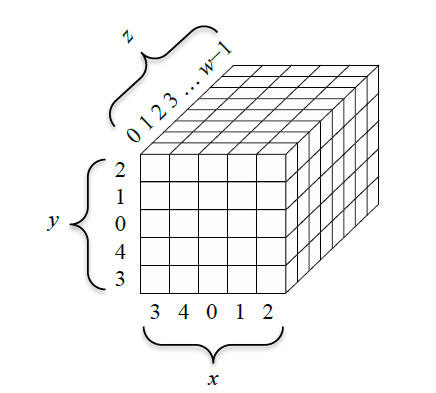
\includegraphics[width=1\linewidth]{figuras/State}
		\caption{\small Dibujo de un vector de estado \cite{FIPS202}.}
		\label{fig:state}
	\end{minipage}\hfill
	\begin{minipage}{0.51\textwidth}
		\centering
		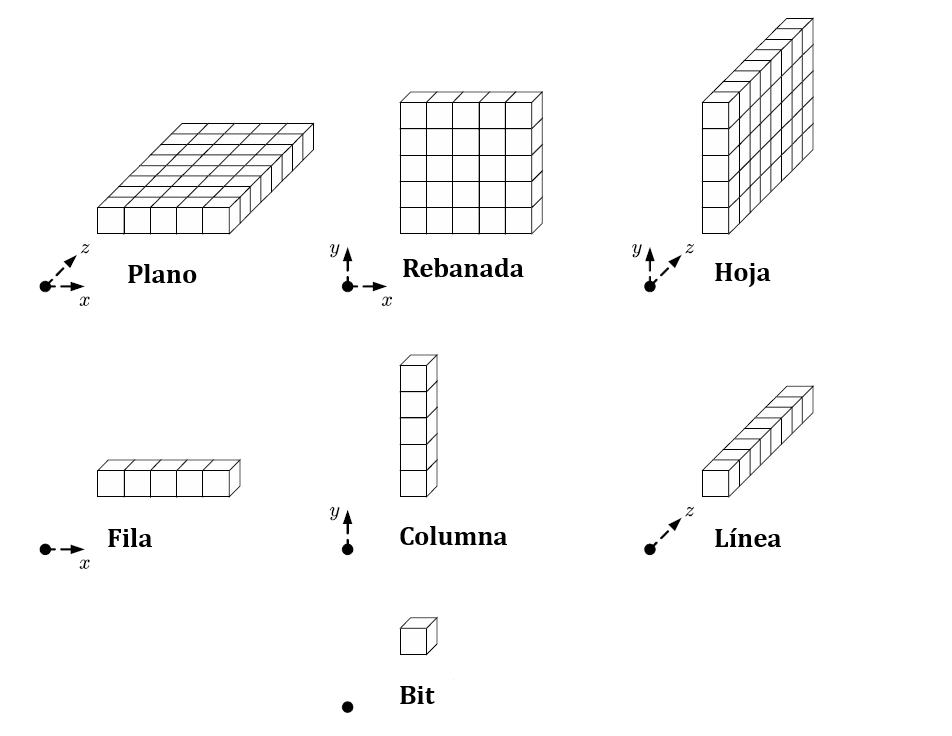
\includegraphics[width=1\linewidth]{figuras/PartsState}
		\caption{ \small Elementos de un vector de estado \cite{FIPS202}.}
		\label{fig:partsstate}
	\end{minipage}
\end{figure}

Para convertir de la cadena \(S\) en la matriz \(A\) se usa la siguiente expresión:
\begin{equation}
	A(x,y,z)=S(w\cdot(5y+x)+z)
\end{equation}

Para convertir de \(A\) a \(S\), se concatenan primero los bits dentro de cada línea, luego las líneas dentro de cada plano y, finalmente, los planos hasta formar la cadena \(S\). Por tanto, si \(||\) denota la concatenación de cadenas, se obtiene:
\begin{equation}
	\begin{array}{lllll}
		\text{Linea}(i,j)=&=A(i,j,0)&||A(i,j,1)&|| \hdots &|| A(i,j,w-1)\\
		\text{Plano}(j)&=\text{Linea}(0,j)&||\text{Linea}(1,j)&|| \hdots &||   \text{Linea}(4,j)\\
		S&=\text{Plano}(0)&||\text{Plano}(1)&||\hdots&|| \text{Plano}(4)
	\end{array}
\end{equation}

Una vez definidos los vectores de estado, estos se manipulan mediante cinco transformadas, denotadas \(\theta\), \(\rho\), \(\pi\), \(\chi\) y \(\iota\). Todas las transformadas toman como entrada un vector de estado \(A(x,y,z)\) y lo transforman, devolviendo un nuevo vector de estado como salida \(A'(x,y,z)\). La transformada $\iota$ recibe además como parámetro el índice de ronda \(i_r\).

\begin{enumerate}
	\item \textbf{Transformada \(\theta\)}: esta transformada realiza una XOR, $\oplus$, del bit \(A(x,y,z)\) con la paridad de las columnas \(\text{C}(x-1 \ \text{mod } 5,z)\) y $\text{C}(x+1 \ \text{mod } 5,z-1 \ \text{mod w} )$. Para ello, sigue los siguientes pasos:
	\newpage
	\begin{algorithm}[H]
		\caption{Transformada \(\theta\) en Keccak-p}
		$\begin{array}{p{\textwidth}}
			\textbf{Entrada: } Matriz \(A\) \\ 
			\hline
			\textbf{Salida: } Matriz \(A'\) \\ 
			\hline
		\end{array}$
		\begin{algorithmic}[1]
			\State Calcular la paridad de cada columna, \(C\):
			\begin{equation}
				C(x,z):=A(x,0,z) \oplus A(x,1,z) \oplus A(x,2,z) \oplus A(x,3,z) \oplus A(x,4,z) 
			\end{equation}
			\State Combinar la paridad de ambas columnas, \(D\):
			\begin{equation}
				D(x,z):=C(x-1 \bmod 5,z) \oplus C(x+1 \bmod 5,z-1 \bmod w)
			\end{equation}
			\State Realizar la XOR con el estado:
			\begin{equation}
				A'(x,y,z):=A(x,y,z)\oplus D(x,z)
			\end{equation}
			\State \Return \(A'\)
		\end{algorithmic}
	\end{algorithm}
	\item \textbf{Transformada \(\rho\)}: esta transformada rota los bits de cada línea un offset módulo la longitud de la línea. Los offsets antes de efectuar el operador módulo se listan en la tabla \ref{tab:rhooffsets}.
	
	\begin{table}[H]
		\centering
		\begin{tabular}{|c|c|c|c|c|c|}
			\hline
			& $x = 3$ & $x = 4$ & $x = 0$ & $x = 1$ & $x = 2$ \\
			\hline
			$y = 2$ & 153 & 231 & 3 & 10 & 171 \\
			\hline
			$y = 1$ & 55 & 276 & 36 & 300 & 6 \\
			\hline
			$y = 0$ & 28 & 91 & 0 & 1 & 190 \\
			\hline
			$y = 4$ & 120 & 78 & 210 & 66 & 253 \\
			\hline
			$y = 3$ & 21 & 136 & 105 & 45 & 15 \\
			\hline
		\end{tabular}
		\caption{Offsets de la transformada $\rho$.}
		\label{tab:rhooffsets}
	\end{table}
	
	Para realizar estas rotaciones sigue los siguientes pasos:
	\begin{algorithm}[H]
		\caption{Transformada \(\rho\) en Keccak-p}
		$\begin{array}{p{\textwidth}}
			\textbf{Entrada: } Matriz \(A\) \\ 
			\hline
			\textbf{Salida: } Matriz \(A'\) \\ 
			\hline
		\end{array}$
		\begin{algorithmic}[1]
			\State Asignar el caso especial de \((x,y,z):=(0,0,z)\):
			\begin{equation}
				A'(0,0,z):=A(0,0,z)
			\end{equation}
			\For{\(t=0:23\)} \Comment{Para los \(23\) valores restantes}
			\State Asignar el valor de la tabla \ref{tab:rhooffsets} modulo \(w\) a cada punto:
			\begin{equation}
				A'(x,y,z):=A(x,y,[z-(t+1)(t+2)/2 \ \text{mod w}])
			\end{equation}
			\State Asignar \((x,y):=(y,2x+3y \ \text{mod } 5)\)
			\EndFor
			\State \Return \(A'\)
		\end{algorithmic}
	\end{algorithm}
	\newpage
	\item \textbf{Transformada \(\pi\)}: esta transformada rota las coordenadas de cada rebanada \((x,y)\) tal como se ilustra en la tabla \ref{tab:piTransform}.
	
	\begin{table}[H]
		\centering
		\begin{tabular}{|c|c|c|c|c|c|}
					\hline
			& $x = 3$ & $x = 4$ & $x = 0$ & $x = 1$ & $x = 2$ \\
			\hline
			$y = 2$ & (4,3) & (0,4) & (1,0) & (2,1) & (3,2) \\
			\hline
			$y = 1$ & (1,3) & (2,4) & (3,0) & (4,1) & (0,2) \\
			\hline
			$y = 0$ & (3,3) & (4,4) & (0,0) & (1,1) & (2,2) \\
			\hline
			$y = 4$ & (0,3) & (1,4) & (2,0) & (3,1) & (4,2) \\
			\hline
			$y = 3$ & (2,3) & (3,4) & (4,0) & (0,1) & (1,2) \\
			\hline
		\end{tabular}
		\caption{Tabla de transformación $\pi$. Para obtener el valor de $A'(x,y)$, se debe leer el valor de la posición $(x',y')$ indicada en la celda correspondiente de la matriz original $A$.}
		\label{tab:piTransform}
	\end{table}
	
	Para realizar esta rotación se sigue el siguiente algoritmo:
	\begin{algorithm}[H]
		\caption{Transformada \(\pi\) en Keccak-p}
		$\begin{array}{p{\textwidth}}
			\textbf{Entrada: } Matriz \(A\) \\ 
			\hline
			\textbf{Salida: } Matriz \(A'\) \\ 
			\hline
		\end{array}$
		\begin{algorithmic}[1]
			\State Calcular la rotación:
			\begin{equation}
				A'(x,y,z):=A(x+3y \ \text{mod } 5,x,z)
			\end{equation}
			\State \Return \(A'\)
		\end{algorithmic}
	\end{algorithm}
	
	
	\item \textbf{Transformada \(\chi\)}: esta transformada actualiza cada bit como el XOR entre el bit original y una combinación no lineal de sus vecinos en la misma fila mediante una puerta AND como se puede ver en la figura \ref{fig:chitransform}.
	
	\begin{figure}[H]
		\centering
		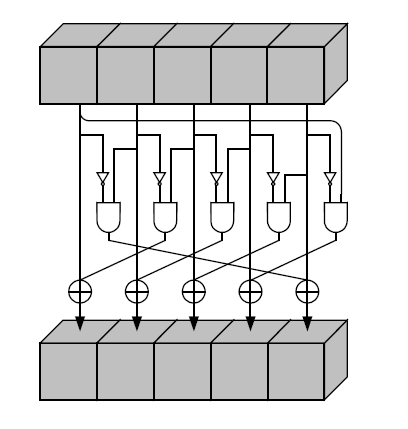
\includegraphics[width=0.4\linewidth]{figuras/PartsState1}
		\caption{Representación de la transformada $\chi$ realizada en cada fila \cite{FIPS202}. Arriba la matriz \(A(x,y,z)\) y abajo la matriz \(A'(x,y,z)\).}
		\label{fig:chitransform}
	\end{figure}
	\newpage
	Para realizar esta rotación se sigue el siguiente algoritmo:
	\begin{algorithm}[H]
		\caption{Transformada \(\chi\) en Keccak-p}
		$\begin{array}{p{\textwidth}}
			\textbf{Entrada: } Matriz \(A\) \\ 
			\hline
			\textbf{Salida: } Matriz \(A'\) \\ 
			\hline
		\end{array}$
		\begin{algorithmic}[1]
			\State Calcular la rotación:
			\begin{equation}
				A'(x,y,z):=A(x,y,z)\oplus\{[A(x+1 \ \text{mod } 5 ,y,z)\oplus 1]\& A(x+2 \ \text{mod } 5 ,y,z)\}
			\end{equation}
			\State \Return \(A'\)
		\end{algorithmic}
	\end{algorithm}
	
	\item \textbf{Transformada \(\iota\)}: esta transformada modifica solo algunos bits de la línea \((0,0)\) de tal manera que que dependa del índice de ronda \(i_r\). Para ello, se sigue el siguiente algoritmo:
	\begin{algorithm}[H]
		\caption{Transformada \(\iota\) en Keccak-p}
		$\begin{array}{p{\textwidth}}
			\textbf{Entrada: } Matriz \(A\) e Índice de ronda \(i_r\) \\ 
			\hline
			\textbf{Salida: } Matriz \(A'\) \\ 
			\hline
		\end{array}$
		\begin{algorithmic}[1]
			\State Asignar:
			\begin{equation}
				A'(x,y,z):=A(x,y,z)
			\end{equation}
			\State Inicializar el vector de ceros \(RC\) de longitud \(w\):
			\For{j=0:l} \Comment{\(l=\log_2(b/25)\) }
			\State Asignar
			\begin{equation}
				RC(2^j-1):=\texttt{rc}(j+7i_r)
			\end{equation}
			\EndFor
			\State Asignar:
			\begin{equation}
				A'(0,0,z):=A'(0,0,z)\oplus RC(z)
			\end{equation} 
			
			\State \Return \(A'\)
		\end{algorithmic}
	\end{algorithm}
	 
	Este algoritmo depende de la función \(\texttt{rc}(t)\)la cual, dado un entero, $t$, genera un bit mediante un procedimiento basado en un registro de desplazamiento con retroalimentación lineal como se describe en el siguiente algoritmo:
	\begin{algorithm}[H]
		\caption{rc}
		$\begin{array}{p{\textwidth}}
			\textbf{Entrada: } Entero \(t\)\\ 
			\hline
			\textbf{Salida: } bir \(rc(t)\) \\ 
			\hline
		\end{array}$
		\begin{algorithmic}[1]
			\If{\(t \ \text{mod } 255 =5\)}
			\State \Return 1
			\EndIf
			\For{i=1:t mod \(255\)}
			\State \(R:=R||R\)
			\State \(R[0]:=R[0]\oplus R[8]\)
			\State \(R[4]:=R[4]\oplus R[8]\)
			\State \(R[5]:=R[5]\oplus R[8]\)
			\State \(R[6]:=R[6]\oplus R[8]\)
			\State \(R:=\texttt{Trunc}_8[R]\) \Comment{Los primeros 8 bits de \(R\)}
			\EndFor
			\State \Return \(R[0]\)
		\end{algorithmic}
	\end{algorithm}
\end{enumerate}
\newpage

Una vez descritas estas transformadas la función de cada ronda, \(\texttt{Rnd}(A,i_r)\) se define como:
\begin{equation}
	\texttt{Rnd}(A,i_r)=\iota(\chi(\pi(\rho(\theta(A)))),i_r)
\end{equation}

Con esta función ya se puede describir el algoritmo \(\texttt{Keccak-p}(b,n_r)\) que consiste en ejecutar \(n_r\) iteraciones de \texttt{Rnd}:

\begin{algorithm}[H]
\caption{Keccak-p}
$\begin{array}{p{\textwidth}}
	\textbf{Entrada: } Cadena \(S\) de longitud \(b\) y Número de rondas \(n_r\) \\ 
	\hline
	\textbf{Salida: } Cadena \(S'\) de longitud \(b\)\\ 
	\hline
\end{array}$
\begin{algorithmic}[1]
	\State Convertir \(S\) en un vector de estado \(A\)
	\For{$i_r$=12+2l-$n_r$:12+2l-1}
	\State A=\texttt{Rnd}$(A,i_r)$
	\EndFor
	\State Convertir \(A\) en una cadena \(S'\) de longitud \(b\)
	\State \Return \(S'\)
\end{algorithmic}
\end{algorithm}
\subsubsection{Función esponja}
Este tipo de función, $\texttt{sponge}[f,pad,r](N,d)$, permite convertir una entrada binaria, \(N\), de cualquier longitud a una salida de longitud \(d\). Para ello, usa tres componentes:
\begin{enumerate}
	\item Una función sobre cadenas de longitud fija, \(f\).
	\item Un parámetro llamado velocidad, \(r\).
	\item Una regla de relleno, \(pad\).
\end{enumerate}
\subsubsection{Seguridad}
\section{Fundamentos de seguridad de los algoritmos}
Al trabajar con algoritmos de cifrado, resulta esencial garantizar su seguridad. Para ello, es necesario establecer con precisión las condiciones que la sustentan. Por ello, a continuación se presentan las definiciones de seguridad relevantes, así como los criterios para la generación de números aleatorios criptográficamente seguros.

\subsection{Indistinguibilidad bajo ataque de texto cifrado adaptable \gls{cca2}}
\cite{CCA2}
\subsubsection{Transformadas Fujisaki-Okamoto \gls{tfo}}
\cite{Fujisaki1999}

\subsection{Generación de números aleatorios criptográficamente seguros}
En esta sección se analiza el proceso de generación de números aleatorios, con el fin de evitar vulnerabilidades que puedan comprometer la seguridad de los algoritmos criptográficos. Un generador predecible permitiría a un atacante inferir los valores producidos, exponiendo así la información de los secretos.
\subsubsection{Generación de números aleatorios en Windows}
\cite{rngWIN}
\subsubsection{Generación de números aleatorios en el PSOC}
\newpage
\section{Funcionamiento básico de los algoritmos postcuánticos}
En esta sección se describe el funcionamiento de los algoritmos postcuánticos analizados en este trabajo. Dado que no se desarrollaron implementaciones propias, sino que se utilizó el código proporcionado por el \gls{nist} en la tercera \cite{nistPQCround3} y cuarta \cite{nistPQCround4} ronda del proceso de estandarización, resulta apropiado presentar su funcionamiento aquí en lugar de en la sección de desarrollo.
\subsection{Fundamentos matemáticos de CRYSTALS-Kyber }
Se utilizará la misma notación empleada en el artículo \cite{kyber-spec-2021}. El conjunto de los enteros sin signo de 8 bits se denota por \(\mathcal{B} = \{0, \dots, 255\}\). Para representar vectores de tamaño \(k\), se utiliza la notación \(\mathcal{B}^k\), mientras que para vectores de tamaño arbitrario se emplea \(\mathcal{B}^*\).
\newline

Para trabajar con estos vectores, se utiliza el símbolo \(||\) para denotar la concatenación de dos cadenas, y la notación \(+k\) para indicar el desplazamiento de \(k\) bytes desde el inicio de una cadena. Por ejemplo, si se tiene una cadena \(a\) de longitud \(l\) y se concatena con una cadena \(b\), se obtiene:
\begin{equation}
	c = a || b
\end{equation}

Entonces:
\begin{equation}
	b = c + l
\end{equation}

Para denotar vectores, se utiliza la notación \(v[i]\), donde \(v\) es un vector columna e \(i\) indica la posición del elemento (empezando desde 0, si no se indica lo contrario). Para las matrices, se emplea la notación \(A[i][j]\), donde \(i\) representa la fila y \(j\) la columna. La transpuesta de una matriz \(A\) se denota como \(A^T\).
\newline

Se denota mediante \(\lfloor x \rceil\) el redondeo de \(x\) al entero más cercano. Por ejemplo: \(\lfloor 2{,}3 \rceil = 2\), \(\lfloor 2{,}5 \rceil = 3\) y \(\lfloor 2{,}8 \rceil = 3\).
\newline

Se denota mediante $\left\| x\right\|$ al valor absoluto de x.
\newline

Para las reducciones modulares se emplean dos tipos: una centrada en cero y otra correspondiente a la reducción modular estándar. Para la reducción modular centrada en cero, sea \(\alpha\) un entero par. Esta operación se define como:
\begin{equation}
	r' = r \ \text{mod}^{\pm} \alpha \quad \Longrightarrow \quad -\dfrac{\alpha}{2} < r' \le \dfrac{\alpha}{2}
\end{equation}

Mientras que la reducción modular estándar se denota como:
\begin{equation}
	r' = r \ \text{mod}^{+} \alpha \quad \Longrightarrow \quad 0 \le r' < \alpha
\end{equation}

Finalmente, se denota mediante \(s \leftarrow S\) la selección de \(s\) de manera uniformemente aleatoria del conjunto \(S\). Si \(S\) representa una distribución de probabilidad, entonces \(s\) se selecciona de acuerdo con dicha distribución.
\newpage

\subsubsection{Transformada Teórica de Números o Number Theoretic Transform (\gls{ntt})}
Para acelerar las operaciones de multiplicación en el esquema basado en retículas, se utiliza la Transformada Teórica de Números (\gls{ntt}, por sus siglas en inglés), la cual permite reducir la complejidad temporal de la multiplicación de polinomios desde \(\mathcal{O}(n^2)\), correspondiente al método tradicional, hasta \(\mathcal{O}(n \log(n))\). Para más detalles, consúltese \cite{cryptoeprint:2024/585}.
\newline

Antes de pasar a explicar el funcionamiento de este método es relevante aclarar que se trabaja sobre el siguiente anillo de polinomios para realizar las operaciones, denotado mediante \(R_q\):
\begin{equation}
	R_q \coloneqq \dfrac{\mathbb{Z}_q[X]}{X^n + 1}
\end{equation}

En la implementación especificada de Kyber, según el artículo \cite{kyber-spec-2021}, se utiliza un valor de \(q=3329\) y \(n=256\). Esta elección es esencial para permitir el uso de la multiplicación mediante la Transformada Teórica de Números (\gls{ntt}), la cual requiere que \(n| (q-1)\), es decir, que \(n\) divida a \((q-1)\). Esta condición garantiza la existencia de \(n\) raíces enésimas de la unidad en \(Z_q\), lo cual es necesario para definir la \gls{ntt}. La validez de esta afirmación se fundamenta en el siguiente teorema\protect\footnotemark[\value{footnote}]:
\newline

\begin{theorem}
	Para \(n\), \(q>1\), el cuerpo  \(Z_q\) tiene una raíz enésima de la unidad si y solo sí \(n| (q-1)\)
\end{theorem} 
\begin{proof}
	Si \(\omega\) es una raíz enésima de la unidad en el conjunto \( \mathbb{Z}_q \), entonces el conjunto:
	\begin{equation}
		\Omega = \left\{1, \omega, \omega^2, \dots, \omega^{n-1} \right\}
	\end{equation}
	forma un subgrupo cíclico \( H \) del grupo multiplicativo \( G_{q-1} \). Por el Teorema de Lagrange, se concluye que el orden de \( H \) divide al orden de \( G_{q-1} \), es decir, \( n \mid (q-1) \).
	\newline
	
	Dado que \( G_{q-1} \) es también un grupo cíclico, existe un generador \(\alpha\) tal que, por el pequeño teorema de Fermat, se cumple:
	\begin{equation}
		\alpha^{q-1} = 1
	\end{equation}
	
	Por lo tanto, el grupo \( G_{q-1} \) puede escribirse como:
	\begin{equation}
		G_{q-1} = \left\{1, \alpha, \alpha^2, \dots, \alpha^{q-2} \right\}
	\end{equation}
	
	Si se define \(\omega\) como:
	\begin{equation}
		\omega = \alpha^{\frac{q-1}{n}},
	\end{equation}
	
	entonces:
	\begin{equation}
		\omega^n = \alpha^{q-1} = 1,
	\end{equation}
	
	y además, para todo \( 0 < k < n \), se cumple:
	\begin{equation}
		k \cdot \frac{q-1}{n} < q-1 \quad \Rightarrow \quad \omega^k \neq 1.
	\end{equation}
	
	Por lo tanto, \(\omega\) es una raíz enésima de la unidad en \(\mathbb{Z}_q\).
\end{proof}
\footnotetext{
	Extraído de la siguiente página web: \url{https://www.csd.uwo.ca/~mmorenom/CS874/Lectures/Newton2Hensel.html/node9.html}
}
\newpage

Por tanto, el polinomio \(X^{256} + 1\) se puede factorizar sobre el cuerpo \(\mathbb{Z}_q\). En la implementación concreta del esquema Kyber, este polinomio se descompone en 128 factores cuadráticos.
\newline

A este polinomio se le aplica la transformada \gls{ntt} a sus coeficientes, la cual no es más que una variación de la \gls{dft} aplicada a cuerpos finitos \(\mathbb{Z}_q\) y aplicada a polinomios de grado \(n\). Para ello, se definen dos operaciones fundamentales:
\begin{enumerate}
	\item La transformada directa:
	\begin{equation}
		\hat{a}_j=\sum_{i=0}^{n-1} \phi^{i\left(2j+1\right)} a_j \ \text{mod} \ q
	\end{equation}
	\item  La transformada inversa:
	\begin{equation}
		a_i=n^{-1} \sum_{j=0}^{n-1} \phi^{-i\left(2j+1\right)} \hat{a}_j \ \text{mod} \ q
	\end{equation}
\end{enumerate}

Donde $\phi$ es un valor tal que $\phi^2=\omega$, con $\omega$ una raíz enésima de la unidad en \(\mathbb{Z}_q\) y \(n^{-1}\) es la inversa multiplicativa de \(n\) en \(\mathbb{Z}_q\).
\newline

A continuación, se presenta un ejemplo extraído de \cite{cryptoeprint:2024/585} para ilustrar su funcionamiento. Sea el polinomio \(G(x)=5+6x+7x^2+8x^3\), cuyo vector de coeficientes es \(g=[5,6,7,8]\). Trabajando en el anillo \(\mathbb{Z}_{7681}\), y tomando $\phi=1925$, se puede calcular la transformada \gls{ntt} \(\hat{g}\). Aplicando luego la transformada inversa, es posible recuperar el vector original \(g\).
\begin{equation}
	\hat{g}=\begin{bmatrix}
		\phi^0 & \phi^1 & \phi^2 & \phi^3\\
		\phi^0 & \phi^3 & \phi^6 & \phi^1\\
		\phi^0 & \phi^5 & \phi^2 & \phi^7\\
		\phi^0 & \phi^7 & \phi^6 & \phi^5\\
	\end{bmatrix} \cdot \begin{bmatrix}
	5\\
	6\\
	7\\
	8
	\end{bmatrix}=\begin{bmatrix}
	1 & 1925 & 3383 & 6468\\
	1 & 6468 & 4298 & 1925\\
	1 & 5756 & 3383 & 1213\\
	1 & 1213 & 4298 & 5756\\
	\end{bmatrix} \cdot \begin{bmatrix}
	5\\
	6\\
	7\\
	8 \end{bmatrix}= \begin{bmatrix}
	2489\\
	7489\\
	6478\\
	6607 \end{bmatrix}
\end{equation}

Aplicando la transformada inversa, donde la inversa de $\phi=1925$ en \(\mathbb{Z}_{7681}\) es $\phi^{-1}=1213$ y el inverso del orden del polinomio \(n=4\) es \(n^{-1}=5761\):
\begin{equation}
	g=n^{-1}\begin{bmatrix}
		\phi^0 & \phi^0 & \phi^0 & \phi^0\\
		\phi^{-1} & \phi^{-3} & \phi^{-5} & \phi^{-7}\\
		\phi^{-2} & \phi^{-6} & \phi^{-2} & \phi^{-6}\\
		\phi^{-3} & \phi^{-1} & \phi^{-7} & \phi^{-5}\\
	\end{bmatrix} \cdot \hat{g}=5761\begin{bmatrix}
	1 & 1 & 1 & 1\\
	1213& 5756& 6468& 1925\\
	4298& 3383& 4298& 3383\\
	5756& 1213& 1925& 6468\\
	\end{bmatrix} \cdot \begin{bmatrix}
	2489\\
	7489\\
	6478\\
	6607 \end{bmatrix}
\end{equation}

Con estas transformadas definidas se define el producto o convolución negativa en el anillo \(	R_q \coloneqq \dfrac{\mathbb{Z}_q[X]}{X^n + 1}\) entre dos polinomios \(g\) y \(h\) como:
\begin{equation}
	g\cdot h= \text{NTT}^{-1}(\text{NTT}(g)\circ\text{NTT}(h))
\end{equation}

Donde la operación \(\circ\) denota la multiplicación elemento a elemento (o punto a punto) entre los vectores en ${Z}_q[X]$.
\newpage

Ahora, queda demostrar que el tiempo de ejecución de la \gls{ntt} es de \(\mathcal{O}(n \log(n))\). Para lograr este cometido, se aprovechan dos propiedades que cumplen estas raíces calculadas:
\begin{enumerate}
	\item Peridicidad: 
	\begin{equation}
		\phi^{k+2n}=\phi^k
	\end{equation}
	\item Simetría:
	\begin{equation}
		\phi^{k+n}=\phi^{-k}
	\end{equation}
\end{enumerate}

Con estas propiedades, se puede implementar el algoritmo de Cooley-Tukey \cite{CooleyALG} que consiste en ir descomponiendo el problema en mitades de manera recursiva para reducir al máximo la cantidad de cálculos realizados. Partiendo de la transformada directa y desarrollando:
\begin{equation}
	\hat{a}_j=\sum_{i=0}^{n-1} \phi^{i\left(2j+1\right)} a_j \ \text{mod} \ q = \sum_{i=0}^{n/2-1} \phi^{4ij+2i} a_{2i} + \phi^{2j+1} \sum_{i=0}^{n/2-1} \phi^{4ij+2i} a_{2i+1} \ \text{mod} \ q
\end{equation}

Si se sustituye \(A_j=\sum_{i=0}^{n/2-1} \phi^{4ij+2i} a_{2i}\) y \(B_j=\sum_{i=0}^{n/2-1} \phi^{4ij+2i} a_{2i+1}\). Ahora aplicando simetría en \(\phi\):
\begin{equation}
	\hat{a}_j=A_j+\phi^{4ij+2i}B_j  \ \text{mod} \ q
\end{equation}
\begin{equation}
	\hat{a}_{j+n/2}=A_j-\phi^{4ij+2i}B_j  \ \text{mod} \ q
\end{equation}

Donde las matrices \(A_j\) y \(B_j\)pueden obtenerse como el resultado de aplicar la \gls{ntt} sobre la mitad de los puntos, gracias a la estructura recursiva del algoritmo. Esto implica que, si \(n\) es una potencia de \(2\), el proceso puede repetirse recursivamente sobre subproblemas de tamaño cada vez menor, hasta alcanzar el caso base. 
\newline

De manera similar, se puede mostrar esta propiedad para la transformada inversa. Por tanto, se demuestra que este algoritmo tiene complejidad \(\mathcal{O}(n \log(n))\).
\newline

En el caso concreto de Kyber \cite{kyber-spec-2021}, la Transformada (\gls{ntt}) de un polinomio en el anillo \(R_q\) se representa como un vector de 128 polinomios de grado 1.
\newline

Sean las 256 raíces enésimas de la unidad \(\left\{\xi, \xi^3, \dots, \xi^{255}\right\}\), con \(\xi = 17\) como primera raíz primitiva. Entonces, se cumple que:
\begin{equation}
	X^{256}+1=\prod_{i=0}^{127}\left(X^2- \xi^{2i+1}\right)
\end{equation}

Aplicando la \gls{ntt} propuesta en \cite{kyber-spec-2021} a un polinomio \(f\in R_q\) se obtiene:
\begin{equation}
	NTT(f)=\hat{f}=\left(\hat{f}_0+\hat{f}_1X,\hat{f}_2+\hat{f}_3X,...,\hat{f}_{254}+\hat{f}_{255}X\right)
\end{equation}

Con
\begin{equation}
	\begin{array}{l}
		\hat{f}_{2i}=\sum\limits_{j=0}^{127} f_{2j}\xi^{\left(2i+1\right)j}\\
		\hat{f}_{2i+1}=\sum\limits_{j=0}^{127} f_{2j+1}\xi^{\left(2i+1\right)j}
	\end{array}
\end{equation}

Donde mediante la transformada directa \gls{ntt} e inversa \gls{ntt}$^{-1}$ se puede realizar el producto de \(f\),\(g\in R_q\) de manera eficiente de la siguiente manera: 
\begin{equation}
	h=f\cdot g = \text{NTT}^{-1}\left[\text{NTT}(f) \circ \text{NTT}(g)\right]
\end{equation}

Siendo \(\hat{h}=\hat{f}\circ\hat{g}=\text{NTT}(f)\circ \text{NTT}(g)\) la multiplicación base definida como:
\begin{equation}
	\hat{h}_{2i}+\hat{h}_{2i+1}X=(\hat{f}_{2i}+\hat{f}_{2i+1})\left(\hat{g}_{2i}+\hat{g}_{2i+1}\right) \ \text{mod} \left(X^2-\xi^{2i+1}\right)
\end{equation}


En la figura \ref{fig:NTTFigure} se puede ver una representación gráfica de como funciona este proceso.
\begin{figure}[H]
	\centering
		\begin{circuitikz}
			\tikzstyle{every node}=[font=\LARGE]
			\draw  (5.25,13.75) rectangle (7.75,12.25);
			\draw  (13.5,13.75) rectangle (16,12.25);
			\node [font=\LARGE] at (6.5,13) {f $\cdot$ g};
			\node [font=\LARGE] at (14.75,13) {h};
			\draw [ color={rgb,255:red,255; green,40; blue,40}, ->, >=Stealth] (7.75,13) -- (13.5,13);
			\node [font=\LARGE, color={rgb,255:red,255; green,0; blue,0}] at (10.5,13.5) {$\mathcal{O}(n^2)$};
			\node [font=\normalsize] at (10.5,12.5) {Multiplicación directa};
			\draw  (5.25,9.5) rectangle (7.75,8);
			\draw  (13.5,9.5) rectangle (16,8);
			\draw [ color={rgb,255:red,0; green,64; blue,255}, ->, >=Stealth] (6.5,12.25) -- (6.5,9.5);
			\draw [ color={rgb,255:red,0; green,64; blue,255}, ->, >=Stealth] (7.75,8.75) -- (13.5,8.75);
			\draw [ color={rgb,255:red,0; green,64; blue,255}, ->, >=Stealth] (14.75,9.5) -- (14.75,12.25);
			\node [font=\LARGE] at (5.75,10.75) {NTT};
			\node [font=\LARGE] at (15.75,10.75) {NTT$^{-1}$};
			\node [font=\LARGE, color={rgb,255:red,0; green,64; blue,255}] at (10.5,9.25) {$\mathcal{O}(n\log(n))$};
			\node [font=\normalsize] at (10.75,8.25) {Multiplicación mediante NTT};
			\node [font=\LARGE] at (6.5,8.75) {$\hat{f}$ $\circ$ $\hat{g}$};
			\node [font=\LARGE] at (14.75,8.75) {$\hat{h}$};
		\end{circuitikz}
	\label{fig:NTTFigure}
	\caption{Representación del cálculo de un producto de polinomios mediante \gls{ntt} en comparación con los algoritmos clásicos.}
\end{figure}


\subsubsection{Aprendizaje Con Errores o Learning With Errors (\gls{lwe})}
Para la elaboración de esta sección, se ha utilizado la información contenida en el artículo \cite{LWElearning}, el cual expone los fundamentos matemáticos del problema de Aprendizaje con Errores (Learning With Errors, \gls{lwe}). Este problema constituye la base teórica sobre la que se sustenta el esquema criptográfico Kyber.
\newline

Para ello, los esquemas basados en \gls{lwe} trabajan con un objeto matemático conocido como retícula. Una retícula es un conjunto discreto de puntos en el espacio, generado por todas las combinaciones lineales con coeficientes enteros de un conjunto de \(n\) vectores linealmente independientes que conforman una base $\mathbb{B}=\left\{b_1,...,b_n\right\}$:
\begin{equation}
	\mathcal{A}=\mathcal{L}(\mathbb{B})= \left\{\sum_{i\in n} z_ib_i: z\in Z^n\right\}
\end{equation}

Esta definición será útil en la demostración de la seguridad de los esquemas basados en \gls{lwe}. Aun así, antes de pasar a la explicación del algoritmo de intercambio de claves públicas, es necesario definir el problema de Aprendizaje con Errores.
\newline

El Aprendizaje con Errores consiste en la tarea de distinguir entre parejas de la forma \((a_i, b_i) \in \mathbb{Z}_q^n \times \mathbb{Z}_q\), donde \(b_i \approx \langle a_i, s \rangle\), y parejas generados de manera completamente aleatoria. Donde, \(s \in \mathbb{Z}_q^n\) es el secreto  que se mantiene fijo para todas las muestras, \(a_i \in \mathbb{Z}_q^n\) es un vector elegido uniformemente al azar, y \(\langle ,  \rangle\) denota el producto escalar Euclídeo.
\newline

La principal utilidad criptográfica del problema \gls{lwe} radica en que, para quien no conoce el secreto, resulta computacionalmente difícil distinguir entre pares estructurados y pares aleatorios. En cambio, quien sí conoce el secreto puede identificar fácilmente qué parejas son consistentes con este, lo que permite construir esquemas seguros de cifrado e intercambio de claves.
\paragraph{\gls{lwe} en anillos}
\mbox{}\\

En Kyber no se parte del problema LWE “puro”, ya que los esquemas basados directamente en \gls{lwe} suelen presentar claves de tamaño y tiempos de cálculo con un orden de magnitud \(\mathcal{O}(n^2)\) \cite{Micciancio2009}. Esto se debe a que, al trabajar con matrices genéricas, se carece de la estructura de anillo necesaria para aprovechar multiplicaciones mediante convolución rápida, es decir, la \gls{ntt}. En cambio, Kyber se fundamenta en una variante conocida como Modulus-LWE (\gls{mlwe}), donde las operaciones de multiplicación matricial se pueden implementar como multiplicaciones de polinomios en $\dfrac{\mathbb{Z}_q[x]}{X^n + 1}$, lo cual permite usar la \gls{ntt}.
\newline


Antes de describir en detalle el funcionamiento de la \gls{mlwe}, conviene introducir primero el problema Ring-LWE (\gls{rlwe}). La \gls{mlwe} puede entenderse como una extensión modular (un vector) de \gls{rlwe}. Este enfoque permite romper la simetría inherente a un anillo y aporta mayor flexibilidad en la selección de parámetros para lograr una mejor relación entre eficiencia y resistencia criptográfica \cite{cryptoeprint:2019/930}.
\newline

En cuanto a la eficiencia en la reducción del tamaño de las claves, esta puede observarse claramente a través del siguiente ejemplo ilustrativo:
\begin{table}[H]
	\centering
	\renewcommand{\arraystretch}{1.2}
	\begin{tabular}{lcc}
		\hline
		Esquema & \gls{lwe} & \gls{rlwe} \\
		\hline
		Tamaño clave pública & \(\mathcal{O}(n^2)\) bits & \(\mathcal{O}(n)\)  \\
		\hline
		Operación para generar la pareja & \(b_i=\langle a_i, s \rangle + e_i\) & \(b[x]=a[x]\cdot s[x]+e[x]\)\\
		\hline
		Matriz \(A\) &$\begin{pmatrix}
							1  &2\\
							3 &4
						\end{pmatrix}$ &3+11X\\
		\hline
		Secreto \(s\) & $\begin{pmatrix}
							5\\
							6
						\end{pmatrix}$&5+6X\\
		\hline
		Error \(e\)& $\begin{pmatrix}
							1\\
							1
						\end{pmatrix}$&1+X\\
		\hline
		Resultado \(b\)&$\begin{pmatrix}
							1\\
							6
						\end{pmatrix}$ & 1+6X\\
		\hline
	\end{tabular}
	\caption{Tabla con un ejemplo numérico del calculo del valor \(b\) necesario para el problema \gls{lwe} como en \gls{rlwe} para ver como efectivamente en la clave pública \((a,b)\) el tamaño es menor. En este ejemplo se trabaja en \(\mathbb{Z}_{17}\) y \(X^2 + 1\). En \gls{mlwe} las claves son de tamaño similar que en \gls{rlwe} pues la matriz \(A\) se puede reconstruir a través de una semilla y la matriz \(b\) solo ve reescalada en función de la seguridad empleada.}
	\label{tab:LWE-RLWE}
\end{table}


\newpage

\paragraph{Aplicación del \gls{rlwe} para el intercambio de claves públicas}
\mbox{}\\

A continuación, se presenta el algoritmo principal empleado para el intercambio de claves basado en el problema \gls{rlwe} que fundamenta matemáticamente el funcionamiento de Kyber. El uso de la \gls{mlwe} es similar y se puede consultar en la sección \ref{sub:kybAlg}.
\newline

El algoritmo de generación de claves emplea los valores \(q\) y \(n\) , que definen la estructura algebraica, para calcular la llave privada \(sk\)  y la llave pública \(pk\).
\begin{algorithm}[H]
	\caption{Generación claves \gls{rlwe} en $\mathbb{Z}_q[x]/(X^n + 1)$ \protect\footnotemark[\value{footnote}]} 
	$\begin{array}{p{\textwidth}}
		\textbf{Entrada: } \(q\), \(n\)\\ 
		\hline
		\textbf{Salida: } \(sk\), \(pk\) \\ 
		\hline
	\end{array}$
	\begin{algorithmic}[1]
		\State Generar \(a\in R_q\)  al azar según una distribución uniforme.
		\State Generar \(sk, e \in R_q\) como elementos pequeños según la distribución del error. \Statex \Comment{Binomial en Kyber, discreta Gaussiana en otros esquemas}
		\State Calcular 
		\begin{equation}
			b:=a\cdot sk + e
		\end{equation}
		\State \Return \((sk, pk:=a||b)\)
	\end{algorithmic}
\end{algorithm}

En el algoritmo de cifrado a partir de la llave pública, \(pk\) y un mensaje \(z\in \{0,1\}^n \) se obtienen los textos cifrados \(u\) y \(v\) que serán enviados al poseedor de la clave privada para descifrar el mensaje. 
\begin{algorithm}[H]
	\caption{Cifrado \gls{rlwe} \protect\footnotemark[\value{footnote}]} 
	$\begin{array}{p{\textwidth}}
		\textbf{Entrada: } \(pk\), \(z\), \(q\), \(n\)\\ 
		\hline
		\textbf{Salida: } \(u\), \(v\) \\ 
		\hline
	\end{array}$
	\begin{algorithmic}[1]
		\State Generar \(r, e_1, e_2 \in R_q\) como elementos pequeños según la distribución del error.
		\State Calcular el primer texto cifrado \(u\):
		\begin{equation}
			u:=a\cdot r + e_1 \ \text{mod}^{+}\text{q}
		\end{equation}
		\State Calcular el segundo texto cifrado \(v\):
		\begin{equation}
			v:=b\cdot r+e_2+\left\lfloor \dfrac{q}{2} \right\rceil \cdot z \ \text{mod}^{+}\text{q}
		\end{equation}
		\State \Return \((u,v)\) 
		 
	\end{algorithmic}
\end{algorithm}

En el algoritmo de descifrado, a partir de los textos cifrados \(u\) y \(v\)se recupera el mensaje original \(z\). La seguridad del esquema radica en el término de ruido ($\varepsilon=r\cdot e- s\cdot e_1 +e_2$) que ofusca el mensaje, el cual solo puede recuperarse correctamente usando la clave secreta siempre que \(\left\|\varepsilon\right\|< q/4\).
\newline

Para mantener este error dentro de niveles aceptables, es fundamental ajustar adecuadamente los parámetros de las distribuciones de ruido en el algoritmo Kyber. En la versión empleada en este trabajo (Kyber1024), esto se traduce en una tasa de error de $2^{-174}$ \cite{pqcrystalssecurity}.
\footnotetext{
	En Kyber se usa la variante \gls{mlwe}, donde
	\(s\in R_q^d\), \(A\in R_q^{d\times d}\) y \(b=A\cdot s + e \in R_q^d\);
	el pseudocódigo completo en \gls{mlwe} aparece en la sección \ref{sub:kybAlg}.
}
\newpage
\begin{algorithm}[H]
	\caption{Descifrado \gls{rlwe} \protect\footnotemark[\value{footnote}]} 
	$\begin{array}{p{\textwidth}}
		\textbf{Entrada: } \(sk\), \(u\), \(v\), \(q\), \(n\)\\ 
		\hline
		\textbf{Salida: } \(z\)\\ 
		\hline
	\end{array}$
	\begin{algorithmic}[1]
		\State Calcular el polinomio \(z'\) a partir del cual se calcula el mensaje.
		\begin{equation}
			\label{eq:ruidoLWE}
			z':=v-u\cdot s = \left(r\cdot e- s\cdot e_1 +e_2\right)+\left\lfloor \dfrac{q}{2} \right\rceil \cdot z \ \text{mod}^{+}\text{q}
		\end{equation}
		\State Calcular la distancia de cada coeficiente \((z'_i)\) de \(z'\):
		\Statex \hspace{1em} \textbf{1.1:} Distancia a \(0\):
		\begin{equation}
			\text{d}_i(0):=\left\| z'_i \ \text{mod}^{\pm} \left\lfloor \dfrac{q}{2} \right\rceil \right\| 
		\end{equation} 
		\Statex \hspace{1em} \textbf{1.2:} Distancia a $\left\lfloor \dfrac{q}{2} \right\rceil$:
			\begin{equation}
			\text{d}_i\left(\dfrac{q}{2}\right)=\left\| \left\lfloor \dfrac{q}{2} \right\rceil - \text{d}_i(0)\right\| 
		\end{equation} 
		\If{$\text{d}_i(0)<\text{d}_i\left(\dfrac{q}{2}\right)$}
			\Statex
			\State Descifrar el bit \(i\) del mensaje \(z\) como un \(0\).
		\Else
			\State Descifrar el bit \(i\) del mensaje \(z\) como un \(1\).
		\EndIf
		\State \Return \(z\)
	\end{algorithmic}
\end{algorithm}
 \footnotetext{
 	En Kyber se usa la variante \gls{mlwe}, donde
 	\(s\in R_q^d\), \(A\in R_q^{d\times d}\) y \(b=A\cdot s + e \in R_q^d\);
 	el pseudocódigo completo en \gls{mlwe} aparece en la sección \ref{sub:kybAlg}.
 }
 En el anexo \ref{chap:ej:rlwe} se puede ver un breve ejemplo de aplicación numérica de funcionamiento de los algoritmos anteriores.

\paragraph{Uso de \gls{mlwe} en Kyber}
\mbox{}\\
A partir del siguiente articulo se define la \gls{mlwe} que es el esquema de fondo en Kyber \cite{cryptoeprint:2019/930}.
\newline

Sean \(R_q\) el anillo a trabajar y \(d\) la dimensión de la retícula. Se define:
\[
\begin{aligned}
	s &\in R_q^d 
	&& \quad \text{(el vector secreto)}\\
	A &\in R_q^{d\times d} 
	&& \quad \text{(la matriz pública, muestreada \(R_q^{d\times d}\) a partir de una semilla $\rho$)}\\
	e &\in R_q^d 
	&& \quad \text{(el vector de error, con coeficientes “pequeños”)}\\
	b &\in R_q^d 
	&& \quad \text{(la pareja resultante)}\\
	b &= A \cdot s + e 
	&& \in R_q^d
\end{aligned}
\]
Entonces, el problema \gls{mlwe} (como extensión modular de \gls{rlwe}) se define como el problema de distinguir muestras \((A, b)\) de parejas uniformes en \(R_q^{d\times d}\times R_q^d\).
\newline

Como se observa, esta definición resulta relativamente sencilla de entender a partir del ejemplo anterior. Sin embargo, las razones que avalan su seguridad son diferentes: al presentar una estructura menos uniforme, la \gls{mlwe} ofrece mejores garantías frente a ataques que explotan la regularidad de los anillos. 
\newline

Por tanto, la \gls{mlwe} es un punto intermedio entre ambos esquemas que permite:
\begin{itemize}
	\item Escalabilidad en seguridad mediante el parámetro $d$.
	\item Mejor eficiencia que en \gls{lwe}, al poder emplear la \gls{ntt} sobre anillos.
	\item Reducción del tamaño de claves, pues la matriz \(A\) puede reconstruirse a partir de una semilla.
	\item Mayor robustez, dado que su estructura “menos simétrica” que un anillo puro dificulta algunos ataques específicos a \gls{rlwe}.
\end{itemize}


\subsubsection{Fundamentos de seguridad de Kyber}
\paragraph{Seguridad esperada en Kyber}
\mbox{}\\
\paragraph{Análisis respecto a ataques conocidos en el esquema Kyber}
\mbox{}\\
\subsubsection{Parámetros empleados en Kyber}
A continuación, se presenta una tabla con los parámetros del esquema Kyber1024 empleado en este trabajo fin de grado.
\begin{table}[h]
	\centering
	\renewcommand{\arraystretch}{1.2}
	\begin{tabular}{lccccccccccc}
		\hline
		&\(n\)&\(k\)&\(q\)&\(\eta_1\)&\(\eta_2\)&\(d_u\)&\(d_v\)&\(\delta\)&\(pk (bytes)\)&\(sk (bytes)\)&\(c (bytes)\)\\
		\hline
		Kyber1024&\(256\)&\(4\)&\(3329\)&\(2\)&\(2\)&\(11\)&\(5\)&\(2^{-174}\)&\(3168 \ (32)\)&\(1568\)&\(1568\)\\
		\hline
	\end{tabular}
	\caption{Tabla con los parámetros utilizados por Kyber1024. El valor de \(n=256\) se elige para permitir una escalabilidad sencilla y permitir distintos niveles de seguridad sin perder capacidad de tener un nivel de ruido aceptable. El valor de \(k=4\) fija el tamaño de la retícula e implica una seguridad de 256 bits. El valor de \(q=3329\) es un primo que satisface \(n|(q-1)\) para permitir la \gls{ntt}, los primos anterior y siguiente que también satisfacen esta propiedad conllevan probabilidades de fallo demasiado altas. Los valores $\eta_1$ y $\eta_2$ definen el ruido y junto a \(d_u\) y \(d_v\) se usan para equilibrar la seguridad y la tasa de fallos $\delta$. El valor \((32)\) en la llave pública es el tamaño de la semilla necesaria para reconstruirla.}
	\label{tab:KyberParams}
\end{table}


\newpage

\subsubsection{Algoritmos principales de Kyber \cite{kyber-spec-2021}}
\label{sub:kybAlg}
El algoritmo de generación de llaves genera las llaves pública \((pk)\) y privada \((sk)\) a partir de los parámetros de la tabla \ref{tab:KyberParams}.

\begin{itemize}
	\item La función $\text{Parse}(x)$ se encarga de convertir cadenas de bits a su representación \gls{ntt} garantizando que los coefientes \(a_i\) sean del tamaño adecuado \(\log_2(q)\approx 11.7\) y no permitiendo desbordamientos \(a_i<q\).
	\item La función $\text{CBD}_\eta(x)$ muestrea el ruido a partir mediante una distribución binomial. Convierte un vector de bits \(B\in\mathcal{B}^{64\eta}\) a un polinomio \(f\in R_q\).
	\item La función $\text{Encode}_k(x)$ convierte de un vector de bits \(B\in\mathcal{B}^{32l}\) a un polinomio \(f\in R_q\).
\end{itemize}
  

\begin{algorithm}[H]
	\caption{Generación llaves en Kyber}
	$\begin{array}{p{\textwidth}}
		\textbf{Salida: } \(pk\in \mathcal{B}^{12\cdot k\cdot n/8+32}\), \(sk\in \mathcal{B}^{24\cdot k\cdot n/8+96}\) \\ 
		\hline
	\end{array}$
	\begin{algorithmic}[1]
		\State Obtener \(d, z\in\mathcal{B}^{32}\) de manera aleatoria usando una distribución uniforme.
		\State Obtener dos nuevos parámetros \(\rho, \sigma\) expandiendo el valor inicial \(d\):
		\begin{equation}
			(\rho, \sigma):=\text{SHA3-512}(d)
		\end{equation}
		\Statex Se crean las matrices para realizar las operaciones de los algoritmos de la  \gls{rlwe}.
		\For{i=0:k-1}
			\For{j=0:k-1}
				\State $\hat{A}[i][j]:=\text{Parse}[\text{SHAKE-128}(\rho,j,i)]$ \Comment{Muestreo matriz en el dominio NTT.}
			\EndFor
		\EndFor
		\State $N:=0$
		\For{i=0:k-1}
			\State $s[i]:= \text{CBD}_{\eta_1}[\text{SHAKE-256}(\sigma,N)]$ \Comment{Muestreo secreto.}
			\State $N:= N+1$
		\EndFor
		\For{i=0:k-1}
			\State $e[i]:= \text{CBD}_{\eta_1}[\text{SHAKE-256}(\sigma,N)]$ \Comment{Muestreo error.}
			\State $N:= N+1$
		\EndFor
		\State Se convierten las magnitudes mediante la NTT para agilizar los cálculos:
		\begin{equation}
				\begin{array}{l}
					\hat{s}:=\text{NTT}(s)\\
					\hat{e}:=\text{NTT}(e)\\
					\hat{t}:=\hat{A}\circ\hat{s}+\hat{e}\\
				\end{array} 	
		\end{equation}
		\State Se calcula la llave pública:
		\begin{equation}
			pk:=\text{Encode}_{12}(\hat{t}\ \text{mod}^{+}\text{q} )||\rho 
		\end{equation}
		\Statex \Comment{Se envía $\hat{b}$ junto con la semilla $\rho$ para el calculo de $\hat{A}$.}
		\Statex \Comment{Así se reduce el tamaño de la clave enviada.}
		\State Se calcula la llave secreta:
		\begin{equation}
			sk:=\text{Encode}_{12}(\hat{s}\ \text{mod}^{+}\text{q} )||pk||\text{SHA3-256}(pk)||z
		\end{equation}
		\Statex \Comment{Se realiza esta concatenación para cumplir la seguridad \gls{cca2} mediante la \gls{tfo}.}
		\State \Return $(pk,sk)$
	\end{algorithmic}
\end{algorithm}
\newpage

En el algoritmo de cifrado Kyber se obtiene el ciphertexto \(c\) a partir de la llave pública \(pk\), un mensaje \(m\) y una semilla aleatoria \(\gamma\) mediante el uso de la \gls{ntt}.
\begin{itemize}
	\item Las funciones $\text{Compress}_q(x,y)$ y $\text{Decompress}_q(x,y)$ se usan para reducir el tamaño de los textos cifrados basándose en el fundamento descrito para los mecanismos basados en la \gls{rlwe}. 
	\item La función $\text{Decode}_k(x)$  convierte de un polinomio \(f\in R_q\) a un vector de bits \(B\in\mathcal{B}^{32l}\).
\end{itemize}

\begin{algorithm}[H]
	\caption{Cifrado Kyber}
	$\begin{array}{p{\textwidth}}
		\textbf{Entrada: } \(pk\in \mathcal{B}^{12\cdot k\cdot n/8+32}\), \(m\in \mathcal{B}^{32}\), \(\gamma\in \mathcal{B}^{32}\)\\ 
		\hline
		\textbf{Salida: } \(c\in \mathcal{B}^{d_u\cdot k\cdot n/8+d_v\cdot n/8}\)\\ 
		\hline
	\end{array}$
	\begin{algorithmic}[1]
		\State Calcular los parámetros necesarios:
		\State \(N:=0\)
		\For{i=0:k-1}
		\State $r[i]:= \text{CBD}_{\eta_1}[\text{SHAKE-256}(\gamma,N)]$ \Comment{Muestreo elemento \(r\).}
		\State $N:= N+1$
		\EndFor
		\For{i=0:k-1}
		\State $e_1[i]:= \text{CBD}_{\eta_2}[\text{SHAKE-256}(\gamma,N)]$ \Comment{Muestreo del primer error.}
		\State $N:= N+1$
		\EndFor
		\State \(e_2[i]:= \text{CBD}_{\eta_2}[\text{SHAKE-256}(\gamma,N)]\) \Comment{Muestreo del segundo error.}
		\State Calcular los valores de los textos cifrados:
		\begin{equation}
			\begin{array}{l}
				\hat{r}:=\text{NTT}(r)\\
				u:= \text{NTT}^{-1}(\hat{A}^T\circ \hat{r})+e_1\\
				v:=\text{NTT}^{-1}(\hat{t}^T\circ \hat{r})+e_2+ \text{Decompress}_q[\text{Decode}_1(m),1]\\
				c_1:=\text{Encode}_{d_u}[\text{Compress}_q(u,d_u)]\\
				c_2:=\text{Encode}_{d_v}[\text{Compress}_q(v,d_v)]
			\end{array}
		\end{equation}
		\State \Return (\(c:=c1||c2\))
	\end{algorithmic}
\end{algorithm}
\newpage

 En el algoritmo de encapsulado Kyber a partir de la llave pública \(pk\) se obtiene el ciphertexto \(c\) y el secreto compartido \(k\). 
\begin{algorithm}[H]
	\small 
	\caption{Encapsulado Kyber}
	$\begin{array}{p{\textwidth}}
		\textbf{Entrada: } \(pk\in \mathcal{B}^{12\cdot k\cdot n/8+32}\)\\ 
		\hline
		\textbf{Salida: } \(c\in \mathcal{B}^{d_u\cdot k\cdot n/8+d_v\cdot n/8}\), \(k\in \mathcal{B}^{*}\)\\ 
		\hline
	\end{array}$
	\begin{algorithmic}[1]
		\State Obtener los valores necesarios a partir de la llave pública:
		\begin{equation}
			\begin{array}{l}
			\hat{t}:=\text{Decode}_{12}(pk)\\
			p:=pk+12\cdot k\cdot n/8
			\end{array} 
		\end{equation}
		\State Calcular la matriz \(\hat{A}^T\) a partir de \(\rho\) codificado en la llave pública.
		\State Obtener \(m'\) de manera aleatoria usando una distribución uniforme.
		\State Obtener los parámetros \(m, \kappa, \gamma\) a partir de \(m'\) y la llave pública:
		\begin{equation}
			\begin{array}{l}
				m:=\text{SHA3-256}(m')\\
				(\kappa,\gamma):=\text{SHA3-512}[m||\text{SHA3-256}(pk)]
			\end{array} 
		\end{equation}
		\State Obtener el ciphertexto:
		\begin{equation}
			c \gets \text{Cifrado Kyber}(pk,m,\gamma)
		\end{equation}
		\State Calcular el secreto compartido:
		\begin{equation}
			k:= \text{SHAKE-256}[\kappa||\text{SHA3-256}(c)]
		\end{equation}
		\State \Return (\(c,k\))
	\end{algorithmic}
\end{algorithm}

En el algoritmo de decapsulado Kyber a partir del ciphertexto \(c\)  y la llave secreta \(sk\) se puede obtener el secreto compartido \(k\).
\begin{algorithm}[H]
	\small
	\caption{Decapsulado Kyber}
	$\begin{array}{p{\textwidth}}
		\textbf{Entrada: } \(c\in \mathcal{B}^{d_u\cdot k\cdot n/8+d_v\cdot n/8}\), \(sk\in \mathcal{B}^{24\cdot k\cdot n/8+96}\)\\ 
		\hline
		\textbf{Salida: } \(k\in \mathcal{B}^{*}\)\\ 
		\hline
	\end{array}$
	\begin{algorithmic}[1]
		\State Obtener los valores descomprimidos \(u\), \(v\) y el valor de la llave secreta \(s\) en el dominio NTT:
		\begin{equation}
			\begin{array}{l}
				u:=\text{Decompress}_q[\text{Decode}_{d_u}(c,d_u)]\\
				v:=\text{Decompress}_q[\text{Decode}_{d_v}(c+d_u\cdot k\cdot n/8,d_v)]\\
				\hat{s}:=\text{Decode}_{12}(sk)
			\end{array}
		\end{equation}
		\State Obtener el mensaje \(m'\) cifrado anteriormente:
		\begin{equation}
			m':=\text{Encode}_1[\text{Compress}_q\left(v-\text{NTT}^{-1}(\hat{s}^T\circ \text{NTT}(u)),1\right)]
		\end{equation}
		\Statex Para Garantizar la seguridad ante ataques de canal lateral se vuelve a calcular el ciphertexto.
		\State Cifrar \(m'\) con la llave pública \(pk\) y el parámetro \(\gamma\) para obtener el ciphertexto \(c'\):
		\begin{equation}
			\begin{array}{l}
				pk:=sk+12\cdot k\cdot n/8\\
				h:=sk+24\cdot k\cdot n/8+32\\
				(\kappa, \gamma):=\text{SHA3-512}[m'||h]\\
				c'\gets \text{Cifrado Kyber}(pk,m',\gamma)
			\end{array}
		\end{equation}
		\State Comparar los textos cifrados obtenidos, añadiendo un nuevo parámetro \(z\) para textos cifrados no válidos.
		\begin{equation}
			z:=sk+24\cdot k \cdot n/8 +64
		\end{equation}
		\If{$c==c'$}
		\State \Return \(K:=\text{SHAKE-256}[\kappa||\text{SHA3-256}(c)]\) \Comment{Mismo secreto compartido.}
		\Else
		\State \Return \(K:=\text{SHAKE-256}[z||\text{SHA3-256}(c)]\) \Comment{No distinguible de llaves válidas.}
		\EndIf
	\end{algorithmic}
\end{algorithm}
\newpage

\subsection{Fundamentos matemáticos de Saber}
Para elaborar esta sección se parte del artículo de Saber adjuntado con la submission al NIST \cite{saber-spec-2020}. En Saber al igual que en Kyber se trabaja en un anillo de la forma:
\begin{equation}
	R_q=\dfrac{\mathbb{Z}_q}{X^n+1}
\end{equation}

Con \(n=256\), pero con la diferencia de que como \(q=2^{13}\), no es posible utilizar la \gls{ntt}, ya que esta requiere un módulo primo adecuado. No obstante, el uso de un módulo en base \(2\) ofrece ciertas ventajas \cite{modlwr} frente a esquemas basados en \gls{mlwe}:
\begin{itemize}
	\item \underline{Uso de \gls{lwr}}: a diferencia de los esquemas basados en \gls{lwe}, donde es necesario muestrear errores desde una distribución aleatoria, en \gls{lwr} el error se introduce mediante redondeo determinista.
	\item \underline{Uso de potencias de \(2\)}: al trabajar con módulos del tipo \(2^k\), las reducciones modulares se pueden implementar de forma eficiente mediante operaciones de desplazamiento de bits (bitshifts), eliminando la necesidad de reducciones modulares explícitas.
\end{itemize}

\subsubsection{Algoritmos de Toom-Cook y Karatsuba}
Dado que en Saber no se cumple la condición \(n|(q-1)\) para poder utilizar la \gls{ntt}, se recurre a los algoritmos de Karatsuba \cite{Karatsuba} y Toom-Cook-4 \cite{ToomCook} para acelerar las multiplicaciones polinómicas. Para ello se sigue la estructura del diagrama de la figura \ref{fig:ToomKara}.
\newline
\begin{figure}[H]
	\centering
	\begin{adjustbox}{width=\linewidth}
	\begin{circuitikz}
		\tikzstyle{every node}=[font=\normalsize]
		\draw  (3.5,12.75) rectangle  node {\normalsize $255\times 255$} (6.25,11.75);
		\node [font=\normalsize] at (4.75,12.5) {};
		\node [font=\normalsize] at (4.75,12) {};
		\draw [ color={rgb,255:red,0; green,17; blue,255}, ->, >=Stealth] (6.25,12.5) -- (8.75,12.5);
		\node [font=\normalsize] at (7.5,13.25) {Toom-Cook-4};
		\node [font=\normalsize] at (4.75,13.25) {};
		\node [font=\normalsize] at (7.5,12.75) {$\mathcal{O}(n^{1.404})$};
		\draw  (8.75,12.75) rectangle  node {\normalsize $63\times 63$} (11.5,11.75);
		\node [font=\normalsize, color={rgb,255:red,0; green,17; blue,255}] at (4,10.25) {$f(X) \cdot g(X)$};
		\draw [ color={rgb,255:red,0; green,17; blue,255}, ->, >=Stealth] (4,10.5) -- (4,11.75);
		\node [font=\normalsize] at (12,12.25) {};
		\draw [ color={rgb,255:red,0; green,17; blue,255}, ->, >=Stealth] (11.5,12.5) -- (14.25,12.5);
		\node [font=\normalsize] at (13,12.75) {$\mathcal{O}(n^{1.404})$};
		\node [font=\normalsize] at (12.75,13.25) {Karatsuba};
		\draw  (14.25,12.75) rectangle  node {\normalsize $15\times 15$} (17,11.75);
		\draw [ color={rgb,255:red,0; green,17; blue,255}, ->, >=Stealth] (17,12.5) -- (19,12.5);
		\draw  (19,12.75) rectangle  node {\normalsize $1\times 1$} (21.75,11.75);
		\node [font=\normalsize] at (18,13.25) {Tradicional};
		\node [font=\normalsize] at (18.25,12.75) {$\mathcal{O}(n^{2})$};
		\draw [ color={rgb,255:red,255; green,0; blue,0}, ->, >=Stealth] (19,12) -- (17,12);
		\draw [ color={rgb,255:red,255; green,0; blue,0}, ->, >=Stealth] (14.25,12) -- (11.5,12);
		\draw [ color={rgb,255:red,255; green,0; blue,0}, ->, >=Stealth] (8.75,12) -- (6.25,12);
		\draw [ color={rgb,255:red,255; green,0; blue,0}, ->, >=Stealth] (5.75,11.75) -- (5.75,10.5);
		\node [font=\normalsize, color={rgb,255:red,255; green,0; blue,0}] at (5.75,10.25) {$h(X)$};
		\node [font=\normalsize, color={rgb,255:red,15; green,15; blue,15}] at (5.125,10.25) {$=$};
	\end{circuitikz}
	\end{adjustbox}
	\label{fig:ToomKara}
	\caption{Representación del cálculo de un producto de polinomios en Saber. Inicialmente, para polinomios de grado 255, se aplica el algoritmo Toom-Cook-4 que reduce los productos a polinomios de grado 63, ya que ofrece el mejor rendimiento asintótico. Sin embargo, conforme disminuye el tamaño de los polinomios, este rendimiento asintótico se vuelve menos eficiente, por lo que se utiliza el algoritmo de Karatsuba para reducir a polinomios de grado 15, y finalmente se realiza el producto mediante multiplicación tradicional de polinomios.}
\end{figure}

El algoritmo de Toom-Cook-4 usado en Saber \cite{toomcook4} para hacer más eficiente la multiplicación de dos polinomios \(c=f\cdot g\) con una complejidad de \(\mathcal{O}(n^{\log_4(7)})\approx\mathcal{O}(n^{1.404})\), sigue los siguientes pasos:
\begin{itemize}
	\item \textbf{Partición}: en este paso se representan los operandos \(f\), \(g\) mediante 4 bloques iguales teniendo en cuenta que \(n-1\) es el grado del polinomio:
	\begin{equation}
		\begin{array}{l}
			h(T)=h(X,T)=h_0(X)+h_1(X)\cdot T+h_2(X)\cdot T^2+h_3(X)\cdot T^3\\
			T=X^{n/4}
		\end{array}
	\end{equation}
	\newpage
	De esta manera, con la introducción de una nueva variable \(T\) se consigue reducir el tamaño efectivo de los polinomios para el paso de la evaluación. La variable \(X\) se utiliza como un parámetro. Aplicado a los polinomios \(f\) y \(g\) con \(n=256\) en Saber:
	\begin{equation}
		\begin{array}{l}
		f(T)=f_0(X)+f_1(X)\cdot T+f_2(X)\cdot T^2+f_3(X)\cdot T^3\\
		g(T)=g_0(X)+g_1(X)\cdot T+g_2(X)\cdot T^2+g_3(X)\cdot T^3\\
		\end{array}
	\end{equation}
	
	Donde cada \(f_i\) y \(g_i\) son polinomios de grado \(63\).
	
	\item \textbf{Evaluación}: se eligen \(7\) puntos \(v_i\) en los que se evalúan ambos polinomios en \(T\). En \cite{toomcook4} se desarrolla un algoritmo eficiente para luego recuperar adecuadamente los coeficientes en la interpolación y para ello, se deben utilizar los siguientes puntos:
	\begin{equation}
		v_i=\left\{\infty, 2, 1, -1, \dfrac{1}{2}, -\dfrac{1}{2},0\right\}
	\end{equation}
	
	De esta manera el producto se convierte en un polinomio de grado \(6\) en \(T\) de la forma:
	\begin{equation}
		c(T)=c_0+c_1\cdot T+c_2\cdot T^2+c_3\cdot T^3+c_4\cdot T^4+c_5\cdot T^5+c_6\cdot T^6
	\end{equation}
	
	Con cada \(c_i\) siendo un polinomio de grado \(126\) de la forma:
	\begin{equation}
		c_i(X)=c_{i,0}+c_{i,1}\cdot X+c_{i,2}\cdot X^2 + ... + c_{i,126}\cdot X^{126}
	\end{equation}
	
	Analizando este polinomio en todos los puntos se obtiene el producto \(c= A_n \cdot \omega\):
	\begin{equation}
		\begin{pmatrix}
			c_6(X)\\
			c_5(X)\\
			c_4(X)\\
			c_3(X)\\
			c_2(X)\\
			c_1(X)\\
			c_0(X)\\
		\end{pmatrix}=
		\begin{pmatrix}
		1 & 0 & 0 &0 &0 &0&1\\
		64 & 32 & 16 &8 &4 &2&1\\
		1&1    &1    &1  & 1 &1 &1\\
		1&  -1  &  1  &-1 &  1&-1 &1\\
		1/64&  1/32  & 1/16   &  1/8& 1/4 &1/2 &1\\
		1/64&  -1/32  & 1/16   &  -1/8& 1/4 &-1/2 &1\\
		0& 0   &    0&  0& 0 &0 &1\\
		\end{pmatrix}\cdot
		\begin{pmatrix}
			\omega_6(X)\\
			\omega_5(X)\\
			\omega_4(X)\\
			\omega_3(X)\\
			\omega_2(X)\\
			\omega_1(X)\\
			\omega_0(X)\\
		\end{pmatrix}
	\end{equation}

	Para implementar las divisiones por potencias de \(2\) en la práctica se utilizan bitshifts. Mientras que para implementar las multiplicaciones de los polinomios de grado 63 se utiliza el algoritmo de Karatsuba.
	\item \textbf{Interpolación}: se resulve el problema de interpolación \(w(v_i)=\omega_i\) invirtiendo la matriz de Vandermonde \(A_n\) generada mediante \(v_i\) y computando el vector de coeficientes \(w=A_n^{-1}c\). 
	\newline
	
	En este problema de interpolación la matriz se tiene precomputada y una vez obtenidas las inversas se reconstruye el polinomio teniendo en cuenta que este producto se repite para cada uno de los 127 coeficientes del polinomio de salida.
	\newline
	
	Por último, se deshace la división en bloques sustituyendo $T=X^{64}$, que equivale a desplazar los coeficientes, y se aplica la reducción modular correspondiente a $X^{256} + 1$.
\end{itemize}
\newpage

El algoritmo de Karatsuba aplica el paradigma de \esquote{divide y vencerás} para multiplicar los polinomios dividiéndolos en dos partes más pequeñas. No obstante, en la implementación de Saber no se usa Karatsuba \esquote{tradicional} pues se divide en cuatro bloques \cite{saber-spec-2020}. Para ello, utilizando los polinomios de grado \(63\) anteriormente divididos en Karatsuba se vuelve a introducir una variable \(T=X^{16}\) para particionar:
\begin{equation}
	\begin{array}{l}
		f=f_0+f_1\cdot T+f_2\cdot T^2+f_3\cdot T^3\\
		g=g_0+g_1\cdot T+g_2\cdot T^2+g_3\cdot T^3\\
	\end{array}
\end{equation}

Entonces su producto queda como:
\begin{equation}
	f\cdot g =\left\{ \begin{array}{l}
		T^{6}\cdot \left(f_3\cdot g_3\right)+\\
		T^{5}\cdot \left(f_3\cdot g_2+f_2\cdot g_3\right)+\\
		T^{4}\cdot \left(f_3\cdot g_1+f_2\cdot g_2+f_1\cdot g_3\right)+\\
		T^{3}\cdot \left(f_3\cdot g_0+f_2\cdot g_1+f_1\cdot g_2+f_0\cdot g_3\right)+\\
		T^{2}\cdot \left(f_2\cdot g_0+f_1\cdot g_1+f_0\cdot g_2\right)+\\
		T^{1}\cdot \left(f_1\cdot g_0+f_0\cdot g_1\right)+\\
		T^{0}\cdot\left(f_0\cdot g_0\right)\\
	\end{array}\right.
\end{equation}


Descomponiendo adecuadamente en \(9\) productos de polinomios más pequeños \(z_i\) de grado \(15\) que se realizan mediante el método tradicional:
\begin{equation}
	\begin{array}{l}
		z_0=f_0\cdot g_0\\
		z_1=f_1\cdot g_1\\
		z_2=f_2\cdot g_2\\
		z_3=f_3\cdot g_3\\
		z_4=\left(f_0+f_1\right)\left(g_0+g_1\right)\\
		z_5=\left(f_0+f_2\right)\left(g_0+g_2\right)\\
		z_6=\left(f_1+f_3\right)\left(g_1+g_3\right)\\
		z_7=\left(f_2+f_3\right)\left(g_2+g_3\right)\\
		z_8=\left(f_0+f_1+f_2+f_3\right)\left(g_0+g_1+g_2+g_3\right)\\
	\end{array}
	\label{eq:kar_decom}
\end{equation}

Con estos términos se puede ver como la ecuación \ref{eq:kar_decom} se puede escribir como una combinación lineal de los términos anteriores:
\begin{equation}
	f\cdot g= C_0+C_1 T+C_2 T^{2}+C_3 T^{3}+C_4 T^{4}+C_5 T^{5}+C_6 T^{6}
\end{equation}

Donde \(C_i\) es:
\begin{equation}
	\begin{array}{l}
		C_0=z_0\\
		C_1= z_4 - z_1 - z_0\\
		C_2=z_5 -z_2-z_0+z_1\\
		C_3=z_8 - \left(z_7+z_6+z_5+z_4\right)+z_3+z_2+z_1+z_0\\
		C_4=z_6 -z_3-z_1+z_2\\
		C_5= z_7 -z_3-z_2\\
		C_6=z_3
	\end{array}
\end{equation}

Es relevante señalar que el algoritmo Karatsuba empleado en Saber tiene la misma complejidad asintótica que el tradicional \(\mathcal{O}(n^{\log_2(3)})\approx\mathcal{O}(n^{1.585})\), demostrable de forma directa mediante el teorema maestro \cite{masterTh}. 
\newline

Una vez hechas estas descomposiciones recursivas se van deshaciendo las particiones hasta llegar al producto deseado. De esta manera, se consigue reducir considerablemente el tiempo de cálculo.
 
 \newpage
 
\subsubsection{Aprendizaje Con Redondeo Modular o Modular Learning With Rounding (\gls{mlwr})} 
Los esquemas basados en la \gls{lwr} \cite{modlwr} emplean operadores de redondeo y, a diferencia de los esquemas de \gls{lwe}, no requieren muestrear ruido de forma explícita, ya que éste se obtiene a partir de escalar y redondear los coeficientes. Por esta razón, en ocasiones se hace referencia a estos esquemas como una variante \esquote{desaleatorizada} de \gls{lwe}. 
\newline

Asimismo, al igual que en el caso de Kyber, con el fin de incrementar la seguridad del esquema y mitigar posibles ataques contra la estructura del anillo, se recurre a la versión modular de la \gls{lwr}, la cual consiste en considerar dicho anillo en un mayor número de dimensiones. 
\newline

Por tanto, el problema de la \gls{mlwr}se formula como la dificultad de distinguir entre parejas de muestras uniformes \((a,u)\) y parejas \((a,b)\) generadas de la siguiente manera:
\begin{equation}
	\begin{array}{l}
		a \leftarrow \mathcal{U}(R_q^{l\times l}) \\ \\
		s \leftarrow \beta_\mu (R_q^{l\times 1})) \\ \\
		b \in R_p^{l\times 1}\\ \\
		b=\left\lfloor \dfrac{p}{q} (A\cdot s)\right\rceil \\ 
	\end{array}
\end{equation}

Donde $\mathcal{U}$ representa una distribución uniforme,  $\beta_\mu$ representa una distribución binomial centrada en $\mu$ y con desviación típica $\sigma=\sqrt{\mu/2}$, y \(l\) es el tamaño de la retícula. Antes de pasar a describir los algoritmos de generación de claves es relevante comentar la definición de la función $\mathtt{bits}(x,i,j)$:
\begin{equation}
	\mathtt{bits}(x,i,j)=[x>>(i-j)]\& (2^j-1) =\left\{\begin{array}{l}
		\dfrac{x}{2^{i-j}}  \ \text{mod}^{+}\text{$2^j$} \ \text{si} \ j\ne i \\ \\
		x  \ \text{mod}^{+}\text{$2^j$} \ \text{si} \ j= i \\ 	
	\end{array}\right.
\end{equation}

En Saber los protocolos de generación de claves se definen de la siguiente manera:
\begin{algorithm}[H]
	\caption{Generación claves \gls{mlwe}} 
	$\begin{array}{p{\textwidth}}
		\textbf{Entrada: } \(q\), \(p\), \(n\), \(l\), \(\mu\)\\ 
		\hline
		\textbf{Salida: } \(sk\), \(b\), \(A\) \\ 
		\hline
	\end{array}$
	\begin{algorithmic}[1]
		\State Muestrear la matriz \(A\in R_q^{l\times l}\) a partir de una distribución uniforme y el secreto \(sk\in R_q^{l\times 1}\) a partir de la distribución \(\beta_\mu\).
		\State Calcular la llave pública \(b\in R_p^{l\times 1}\):
		\begin{equation}
			b:=\texttt{bits}(A\cdot s + h,\varepsilon_q, \varepsilon_p)
		\end{equation}
		\State \Return \((sk, b, A)\)
	\end{algorithmic}
\end{algorithm}

En este algoritmo los valores $\varepsilon_i$ representan el valor \(\varepsilon_i=\log_2 (i)\) mientras que \(h\in  R_q\) es un polinomio con todos sus coeficientes con iguales a \(2^{\varepsilon_q-\varepsilon_p-1}\) para emular el comportamiento del redondeo.

\begin{algorithm}[H]
	\caption{Cifrado \gls{mlwr}} 
	$\begin{array}{p{\textwidth}}
		\textbf{Entrada: } \(pk\), \(A\), \(q\), \(p\), \(t\), \(n\), \(l\), \(\mu\)\\ 
		\hline
		\textbf{Salida: } \(ss'\), \(b'\), \(c\) \\ 
		\hline
	\end{array}$
	\begin{algorithmic}[1]
		\State Muestrear otro secreto \(s'\in R_q^{l\times 1}\) a partir de la distribución \(\beta_\mu\).	
		\State	Calcular el ciphertexto \(b' \in R_p^{l\times 1}\) y la variable intermedia \(v'\in R_p\) a partir de la matriz \(A\) y la llave pública \(b\):
		\begin{equation}
			\begin{array}{l}
				b':=\texttt{bits}(A^T\cdot s'+h,\varepsilon_q,\varepsilon_p) \\
				v':=b \cdot \texttt{bits}(s',\varepsilon_p,\varepsilon_p)+ h_1 
			\end{array}
		\end{equation}
		\State Calcular el otro ciphertexto \(c\in R_t\) a partir de la variable \(v'\):
		\begin{equation}
			c:=\texttt{bits}(v',\varepsilon_p -1,\varepsilon_t)
		\end{equation}
		\State Calcular el secreto compartido \(ss\)
		\begin{equation}
			ss':=\texttt{bits}(v',\varepsilon_p,1)
		\end{equation}
		\State \Return \((ss', b', c)\)
	\end{algorithmic}
\end{algorithm}

En este algoritmo se generan los ciphertextos para que en el descifrado se obtenga el mismo secreto compartido. El valor \(h_1\in  R_q\) es un polinomio con todos sus coeficientes con iguales a \(2^{\varepsilon_q-\varepsilon_p-1}\) para emular el comportamiento del redondeo.

\begin{algorithm}[H]
	\caption{Descifrado \gls{mlwr}} 
	$\begin{array}{p{\textwidth}}
		\textbf{Entrada: } \(sk\), \(b'\), \(c\), \(p\), \(t\)\\ 
		\hline
		\textbf{Salida: } \(ss\)\\ 
		\hline
	\end{array}$
	\begin{algorithmic}[1]
		\State Calcular la variable intermedia \(v\in R_p\)
		\begin{equation}
			v:=b'^T \cdot \texttt{bits}(s,\varepsilon_p,\varepsilon_p)+ h_1 
		\end{equation}
		\State Calcular el valor del secreto compartido \(ss\)
		\begin{equation}
			ss:=\texttt{bits}(v-2^{\varepsilon_p-\varepsilon_t-1}\cdot c+ h_2),\varepsilon_p,1
		\end{equation}
		\State \Return \(ss\)
	\end{algorithmic}
\end{algorithm}

El valor \(h_2\in  R_q\) es un polinomio con todos sus coeficientes con iguales a \(2^{\varepsilon_p-2}-2^{\varepsilon_p-\varepsilon_t-2}\) para emular el comportamiento del redondeo. Es relevante destacar que para FireSaber \cite{saber-spec-2020}, el valor de las constantes corresponde a los de la tabla \ref{tab:SaberParams}, con los cuales se logra una baja probabilidad de fallo.
\newline

Una vez definidos los algoritmos basados en \gls{mlwr} para el intercambio de claves en Saber, resulta fundamental demostrar que ambas partes obtienen efectivamente el mismo secreto compartido.  Siguiendo el análisis de \cite{Correctness}, la probabilidad de coincidencia del secreto depende de la distancia entre las variables \(v\) y \(v'\). En particular, se cumple que
\begin{equation}
	d = \|v - v'\| \quad \Rightarrow \quad
	\begin{cases}
		d > \dfrac{p}{4}\left(1+\dfrac{1}{t}\right) = c_1, & \text{el secreto difiere}. \\[2ex]
		d < \dfrac{p}{4}\left(1-\dfrac{1}{t}\right) = c_2, & \text{el secreto coincide}. \\[2ex]
		c_2 \leq d \leq c_1, & \text{el secreto coincide con probabilidad intermedia}.
	\end{cases}
\end{equation}

Si se le añade a $\Delta v = v-v'$ una distribución de error \(e_r \in R_p\) en el rango \([-p/4t,p/4t)\), se puede calcular la probabilidad \(1-\delta\) de que ambas partes lleguen al mismo secreto compartido como:
\begin{equation}
	\label{eq:Frodo}
	1-\delta= \text{Pr}\left[\|\Delta v + e_r\|< \dfrac{p}{4}\right]
\end{equation}

En la \gls{mlwr} esta probabilidad se generaliza para que se exprese unicamente en función de las distribuciones de error como se puede ver en el siguiente teorema.

\begin{theorem}
 Sea una \(A\) una matriz en \(R_q^{l\times l}\), \(s\), \(s'\) vectores en \(R_q^{l\times 1}\) muestreados como se describe en los algoritmos anteriores. Se definen \(e\) y \(e'\) como los errores de redondeo introducidos al reescalar y redondear \(A\cdot s\) y \(A^T\cdot s'\), es decir:
 \begin{equation}
 	\label{eq:bitsec}
 	\begin{array}{l}
 		\texttt{bits}(A\cdot s+h,\varepsilon_q,\varepsilon_p)=\dfrac{p}{q}\cdot A\cdot
 		s +e\\\\
 		\texttt{bits}(A^T\cdot s'+h,\varepsilon_q,\varepsilon_p)=\dfrac{p}{q}\cdot A^T\cdot
 		s' +e'\\
 	\end{array}
 \end{equation}
 
 Sea \(e_r  \in R_q\) in polinomio con los coeficientes distribuidos uniformemente en el rango \([-p/4t,p/4t]\). Si se define:
 \begin{equation}
 	\label{eq:probrefeSab}
 	\delta = \text{Pr}\left[\left\|\left(s'^T\cdot e-e'^T\cdot s+ e_r\right) \ \text{mod}^{+}\text{p}  \right\|_\infty > \dfrac{p}{4}\right]
 \end{equation}
 
 entonces tras ejecutar el protocolo de intercambio de claves en Saber, ambas partes acuerdan un secreto compartido de n-bits con probabilidad \(1-\delta\).
\end{theorem} 
\begin{proof} En la demostración de este teorema se utilizan dos pasos, el primero \cite{modlwr} para demostrar  que las condiciones propuestas son equivalentes a las de la ecuación \ref{eq:Frodo} y el segundo paso de elaboración propia para efectivamente mostrar que ambos secretos coinciden:
	\newline
	
	\textbf{Paso 1: Equivalencia de condiciones}  
	\smallskip
	Se despejan los valores de \(b\) y \(b'\) mediante la ecuación \ref{eq:bitsec}:
	\begin{equation}
		\begin{array}{l}
			b=\dfrac{p}{q}\cdot A\cdot s +e \\ \\
			b'=\dfrac{p}{q}\cdot A^T\cdot s' +e'
		\end{array}	
	\end{equation}
	
	A continuación se despejan \(v\) y \(v'\):
	\begin{equation}
		\begin{array}{l}
			v=\dfrac{p}{q}s'^T\cdot A\cdot s +h_1+s'^T\cdot e \ \text{mod}^{+}\text{p}  \\ \\
			v'=\dfrac{p}{q}s'^T\cdot A\cdot s +h_1 +e'^T\cdot s \ \text{mod}^{+}\text{p}
		\end{array}	
	\end{equation}
	
	Simplemente restando se obtiene $\Delta v$ y se claramente se ve la equivalencia a la ecuación \ref{eq:probrefeSab}.
	\newline
	
	\textbf{Paso 2: Igualdad de secretos} 
	\smallskip
	En este paso se hace la demostración empleando los parámetros de FireSaber de la tabla \ref{tab:SaberParams}. Sea \(Q_8 \in R_{128}\):
	\begin{equation}
		Q_8=\left\lfloor \dfrac{v'}{8} \right\rfloor
	\end{equation} 
	
	Como se puede definir \(v'\) a través del operador redondeo hacia abajo si se tiene en cuenta un resto \(r \in R_8\):
	\begin{equation}
		v'=8\left\lfloor \dfrac{v'}{8} \right\rfloor + r
	\end{equation}
	
	Teniendo en cuenta que \(c\) se encuentra en \(R_{64}\) existe un bit de información, \(\omega\), de \(Q_8\) que se esta perdiendo y por tanto, se cumple que:
	\begin{equation}
		c=\left\lfloor \dfrac{v'}{8} \right\rfloor \ \text{mod}^{+}{64}=64\cdot\omega+\left\lfloor \dfrac{v'}{8} \right\rfloor \ \text{mod}^{+}{64}
	\end{equation}
	
	Por tanto, el primer secreto compartido \(ss'\) se puede expresar como:
	\begin{equation}
		ss'=\left\lfloor \dfrac{8\cdot (64\cdot \omega+c)+r}{512} \right\rfloor \ \text{mod}^{+}{2}=\left\lfloor \omega +\dfrac{8\cdot c+r}{512} \right\rfloor \ \text{mod}^{+}{2}
	\end{equation}
	
	Donde como \(c < 64\) y \(r < 8\) se obtiene que este secreto solo depende de $\omega$:
	\begin{equation}
		ss'=\left\lfloor \omega +\dfrac{511}{512} \right\rfloor \ \text{mod}^{+}{2}= \omega \ \text{mod}^{+}{2}
	\end{equation}
	
	Ahora solo queda comprobar que efectivamente el secreto compartido \(ss\) también acaba teniendo este valor. Partiendo de la definición de \(ss\):
	\begin{equation}
		ss=\left\lfloor \dfrac{v-8\cdot c+ h_2}{512}\right\rfloor \ \text{mod}^{+}{2}
	\end{equation}
	
	Sustituyendo \(v\) mediante la definición $\Delta v= v - v'$ y teniendo en cuenta el desarrollo realizado para \(v'\) realizado en las ecuaciones anteriores se obtiene:
	\begin{equation}
		ss=\left\lfloor \dfrac{[8\cdot(64\cdot \omega+c)+r+\Delta]-8\cdot c+ h_2}{512}\right\rfloor \ \text{mod}^{+}{2}
	\end{equation}
	
	Despejando:
	\begin{equation}
		ss=\left\lfloor \omega +\dfrac{r+\Delta+ h_2}{512}\right\rfloor \ \text{mod}^{+}{2}
	\end{equation}
	
	Donde justamente si se hace el cambio de notación \(e_r:=r\) se obtiene la condición de la ecuación \ref{eq:probrefeSab}, el método falla si:
	\begin{equation}
		e_r+\Delta > (512-h_2)= 260 >\dfrac{p}{4}=256
	\end{equation}
\end{proof}
\subsubsection{Fundamentos de seguridad de Saber}
\paragraph{Seguridad esperada en Saber}
\mbox{}\\
\paragraph{Análisis respecto a ataques conocidos en el esquema Saber}
\mbox{}\\
\subsubsection{Parámetros empleados en Saber}
A continuación, se presenta una tabla con los parámetros del esquema FireSaber empleado en este trabajo fin de grado.
\begin{table}[H]
	\centering
	\renewcommand{\arraystretch}{1.2}
	\begin{tabular}{lcccccccccc}
		\hline
		&\(n\)&\(l\)&\(q\)&\(p\)&\(t\)&\(\mu\)&\(\delta\)&\(pk (bytes)\)&\(sk (bytes)\)&\(c (bytes)\)\\
		\hline
		FireSaber&\(256\)&\(4\)&\(2^{13}\)&\(2^{10}\)&\(2^{6}\)&\(6\)&\(2^{-165}\)&\(1312\)&\(3040 \ (1760)\)&\(1472\)\\
		\hline
	\end{tabular}
	\caption{Tabla con los parámetros utilizados por FireSaber. Se elige el valor \(n=256\) para permitir la escalabilidad de Saber mediante el parámetro \(l=4\), que marca el tamaño de las matrices sobre las que se trabaja \(R_q^{k\times k}\). Los parámetros \(q\), \(p\) y  \(t\) tienen esos valores para que la probabilidad de fallo \(\delta\) sea baja. El valor \(\mu\) representa el tamaño de la binomial a partir de la cual se muestrea la llave secreta \(sk\).}
	\label{tab:SaberParams}
\end{table}

\subsubsection{Algoritmos principales de Saber \cite{saber-spec-2020} }
\subsection{Hamming Quasi-Cyclic (\gls{hqc}}
Para  \cite{hqc-spec-2022}
\subsubsection{Fundamentos de seguridad de \gls{hqc}}
\paragraph{Seguridad esperada en \gls{hqc}}
\mbox{}\\
\paragraph{Análisis respecto a ataques conocidos en el esquema \gls{hqc}}
\mbox{}\\
\subsubsection{Parámetros empleados en \gls{hqc}}
\subsubsection{Algoritmos principales de \gls{hqc} \cite{hqc-spec-2022}}

